%	Copyright (C) 2013 Systems Engineering Group
%
%	CHANGELOG:
%       2005-10-10 - corrected and extended. 
%       2013-01-28 - adjusted sections and explanation
%		2020-11-18 - basic content of hand-in


\documentclass[a4paper,10pt,twoside]{article}
\pagestyle{headings}
\usepackage{a4wide}
\usepackage{graphicx}
\usepackage[utf8]{inputenc}
\usepackage[english]{babel}
\usepackage{csquotes}
\graphicspath{ {./images/} }
\usepackage[colorlinks,hyperfigures,backref,bookmarks,draft=false]{hyperref}

\title{Disaggregated Compute and Storage for Distributed LSM-based Databases}
\author{Zidi Chen}
\date{\today}

\begin{document}

\maketitle

\begin{abstract}
Here you provide a very short intoduction into your topic and sum up your hand-in. 
It is important to highlight the main issues to be discussed in your hand-in here.
\end{abstract}

\tableofcontents

\section{Introduction of the Research Field}

Distributed databases like MongoDB, TiDB have been more widely used in many large-scale services senarios.
But in many cases, distributed databases could suffer performace degradation and low utilizationn from skew, backgroud operatio and compaction.
The paper~\textit{Hailstorm: Disaggregated Compute and Storage for Distributed LSM-based Databases} \cite{mainpaper}introduces Hailstorm, a system that disaggregates storage and compute for distributed LSM-based databases.
It shows that Hailstorm achieves load balance in many MongoDB deployments with skewed workloads, improving the average throughput by 60$\%$, while decreasing tail latency by as much as 5×.


\section{Basics}

\subsection{LSM-Tree}

Traditional disk-based index structures such as the B-tree will effectively double the I/O cost of the transaction to maintain an index such as this in real time, increasing the total system cost up to fifty percent. 
Hence Log-structured merge tree (LSM-Tree) \cite{LSM-tree} has been widely used by many distributed databases, as it provides efficient indexing for a key-value store with a high rate of inserts and deletes.
The LSM-tree uses an algorithm that defers and batches index changes, cascading the changes from a memory-based component through one or more disk components in an efficient manner reminiscent of merge sort. 
During this process all index values are continuously accessible to retrievals (aside from very short locking periods), either through the memory component or one of the disk components.

\subsection{Compaction in LSM KV Stores}

Compaction is a critical mechanism in a system based on LSM-Tree. 
Log append method brings high-throughput writes. 
As the sstable continues to be written, more and more files will be opened by the system, and the accumulated data changes (updates, deletes) operations for the same key will increase. 
Since sstable is immutable, the data in the memory will reaches the upper limit in certain layer.
In order to reduce the number of files and clean up invalid data in time, the compaction mechanism was introduced to optimize read performance and space.
\par
Compaction can be implemented in many ways. For example, RocksDB implements Tiered+Leveled, termed Level compaction.\cite{RocksDB_compaction_algo1}. 
\par
Generally, in LSM tree, each level contains multiple partitions of data sorted by keys. When  compaction will be triggered by continuously recycling old version data and merging multiple layers into one layer through periodic background tasks.
The basic procedure goes as following:
\begin{figure}[h]
    \centering
	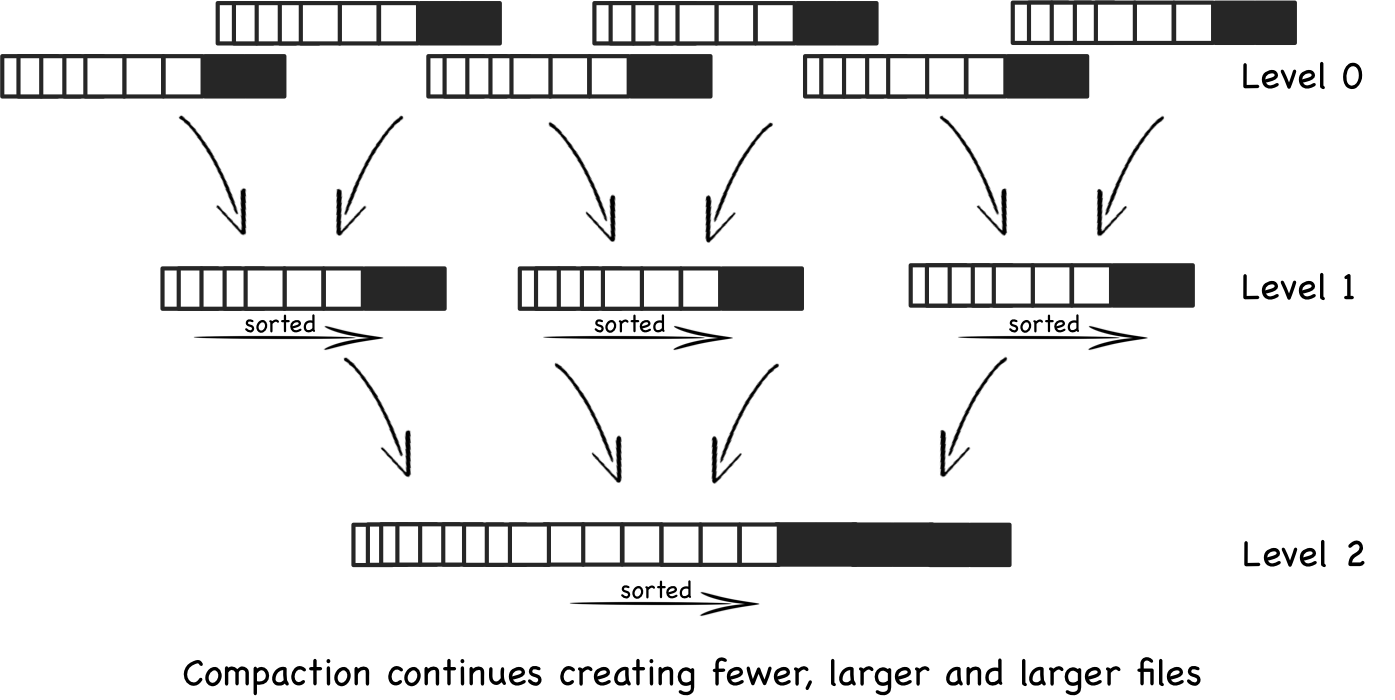
\includegraphics[scale=0.3]{LSM_Tree1.png}
    \caption{LSM Tree}
    \label{fig:mesh1}
\end{figure}
\par
As is shown in Figure. Compaction into level N (L(n)) merges data from L(n-1) to L(n), where data is rewirted into the new level. 
In original paper of LSM tree, all data from L(n-1) is merged into L(n). 
In morden distributed databases such as LevelDB and RocksDB, overlapping data is eliminated, therefore for most time, only some data will be merged into new level.
\par
Generally, LSM tree will continuously compact key-value pairs ,and the compaction and disk flushes will trigger big writes, which will cause significantly overheads due to I/O amplifications.


\subsection{Tow-level Sharding}
Sharding is widely used in distributed databases. Large data sets or high throughput applications can challenge the capacity of one single server.
Each area has the same schema and columns, but each table has completely different rows. 
Similarly, the data stored in each partition is unique and has nothing to do with the data stored in other partitions.
Sharding divides a piece of data into two or more smaller blocks, called logical shards.
Then, logical shards are distributed on separate database nodes, called physical shards.
Physical shards can hold multiple logical shards. 
Nevertheless, the data stored in all shards collectively represent the entire logical data set.
\par
A tow-level sharding way is introduced in the paper\cite{mainpaper}. 
Hailstorm uses a tow-step data assignment scheme, where data objects are dynamically assigned to different partitions, 
so that the system could react better to the changes in the workfload and perform better load balance.
The target LSM-based databases still use the filesystem solution to redistribute data blocks into different nodes uniformly.


\subsection{Skew in Distributed Databases}

Distributed databases \cite{mongodb,tidb} are designed for large-scale data storage, which usually run on multiple nodes in the same,
or even partitioned networks.
Distributed database use sharding to tore larger dataset and handle additional requests by distributing the data among multiple machines.
The database engine translates user queries into individual queries that are routed to one or multiple database instances for execution.
Therefore, the database may suffer skew issue, where keys are unevenly to different nodes, which could cause uneven access and some nodes may become the hotsopt.
This could lead to globally performance degradation.



\section{Previous and Related Work}

\subsection{Skew in Distributed Databases}

Previously proposed solutions to eliminate skew in several ways.
MongoDB introduces a balancer to mitigate imbalanced shards\cite{MongoDB_balancing1}.
Some manual operations can also be performed, e.g., moving "hotspot" chunks manually to address the imbalances. 
In practice, some table related operations will also work, e.g., spliting one table into several sub-tables.
\par
Resharding could be carried out manually or automatically to reduce the influence on performance due to skew.
Auto-splitting is a mechanism in MongoDB\cite{MongoDB_sharding1} that detect automatically when data overflow happens in chunks, 
and then split the oversized chunk into smaller pieces.
The server that runs MongoDB contains the process ChunkSplitter that runs continuously to detect weather any chunk grows beyond the configured chunk size (maxChunkSizeBytes) due to some insert operation.
\par
The auto split task will be carried out if possible and necessary. ChunkSplitter supports asynchronous auto-split, thus, 
multiple split operations could be handled concurrently with no overlap. 
Basic proceduce goes as following: 
First, ChunkSplitter will set the flag to the chunks which need resharding, where the estimated data size will be reset to handle the potiential in-coming writing operations.
Then the splitVector will perform the split by inserting the split keys to original chunk vector, and returning the split points.
\par
Auto-split may not be enough to handle skew issue, as it requires additional operations to reduce read operation hot spots.
So MongoDB uses top chunk optimization to prevent some top chunks becoming potential hot spot.
The balancer ties to move the top chunk out of the shart when auto-split is carried out.
MongoDB also provides auto-balancing mechanism that try to reduce hot spot chunks, where a balancer process runs continuously in the backgroud to monitor the chunk distribution in the cluster.
Resharding operation may still cause some performance loss, some manual operations that takes the structure of the table in consideration may be costly in time.

\subsection{Compaction and performance degradation}
Compaction may cause severe I/O performance degradation in LSM-based distributed databases, 
as it merges multiple tables and writes back to disk, which will typically comsue large I/O and CPU computing resources.
A benchmark test is conducted in the paper\cite{mainpaper}, 
\begin{displayquote}
	Profiling this particular experiment
	reveals that storage is saturated as I/O bandwidth remains
	almost constantly close to 320 MB/s, the maximum write
	bandwidth for our SSD. We also observe peaks of CPU utilization
	when compaction tasks run. 
\end{displayquote}
\begin{figure}[h]
    \centering
	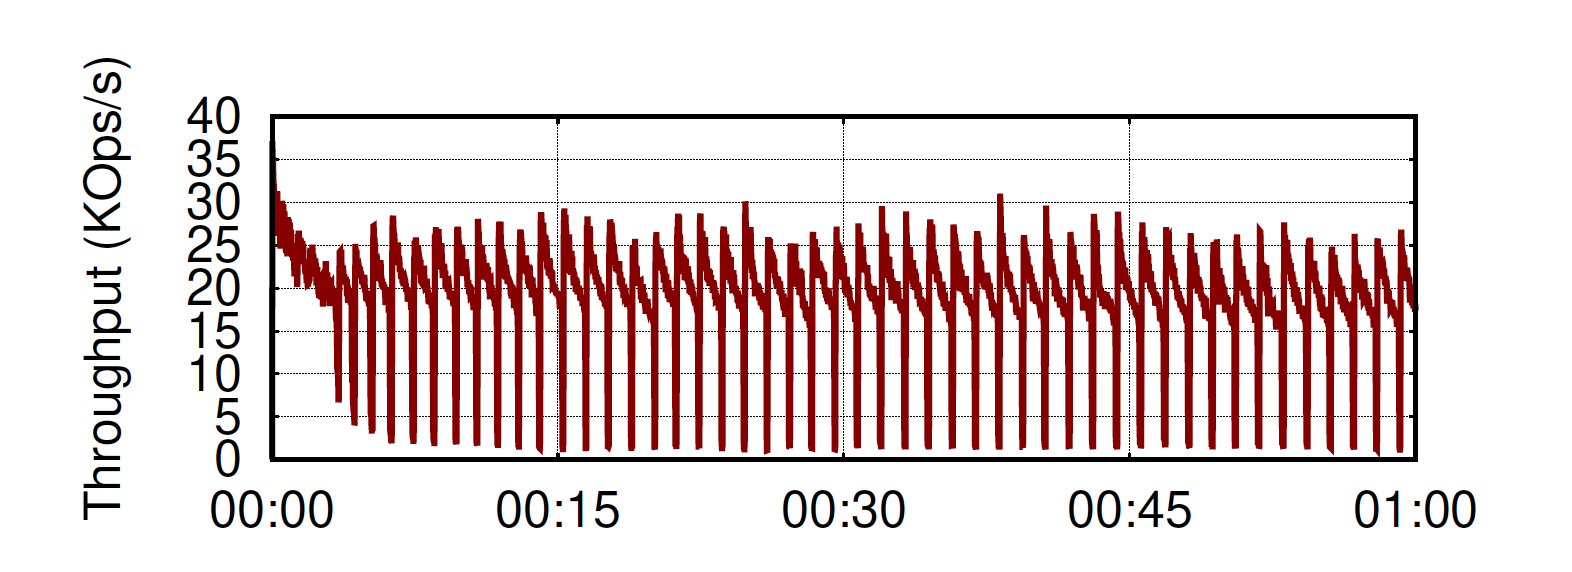
\includegraphics[scale=0.3]{Campaction perf.png}
    \caption{Embedded RocksDB throughput over time (HH:mm) on
	a node equipped with an Intel S3500 Series SSD using the YCSB
	A [38] workload (50$\%$ reads and 50$\%$ writes).}
    \label{fig:mesh1}
\end{figure}

\subsubsection{Light-weight LSM Tree}
The light-weight compaction tree(LWC-Tree) \cite{Yao2017ALC} is a variant from the original LSM tree. 
The LWC-Tree tries to improve the write preformance during compaction by merging a little metadata rather than perform the operation on the while range of data.
As is discussed previously, traditional lSM tree carries out compaction by read, sort and rewrite all whole tables. 
\par
LWC-Tree divides the overlapping data from the original table into small segments, and then appends these segments into the tables on the next level, 
and then only merge related metadata, which is a very small scale compared to the original scale. 
LWC-Tree organizes the DTable structure based on the change of metadata. 
LWC-Tree also provides load balancing for the same level DTables to reduce hot spots as much as possible. 
The balancer moves the overly-full tables data to other tables on the same level by adjusting the key range, which reduces the cost for data movement as much as possible.


\subsubsection{Reducing Involved Components in Compaction}
Skip-tree \cite{7569086} solve the performance degradation caused by compaction in a quite aggresive way.
As is discussed, I/O performance gets severe influence by the compaction due to heavily read and write-to-disk operations.
So Skip-tree skips some components in compaction and put the output of the compaction into some larger components.
The basic architecture of Skip-tree is shown in Figure 3.
Skip-tree introduces a large size memory to store the index for the KV objects as a buffer.
It push the KV objects into non-adjacent components via skipping components during the precedure of compaction as many as possible.
This would reduce the steps of operations from memory to larger disk components, which reduces the I/O throughput.
As a result, there will be fewer compactions before the KV objects reach the destination component.
\begin{figure}[h]
    \centering
	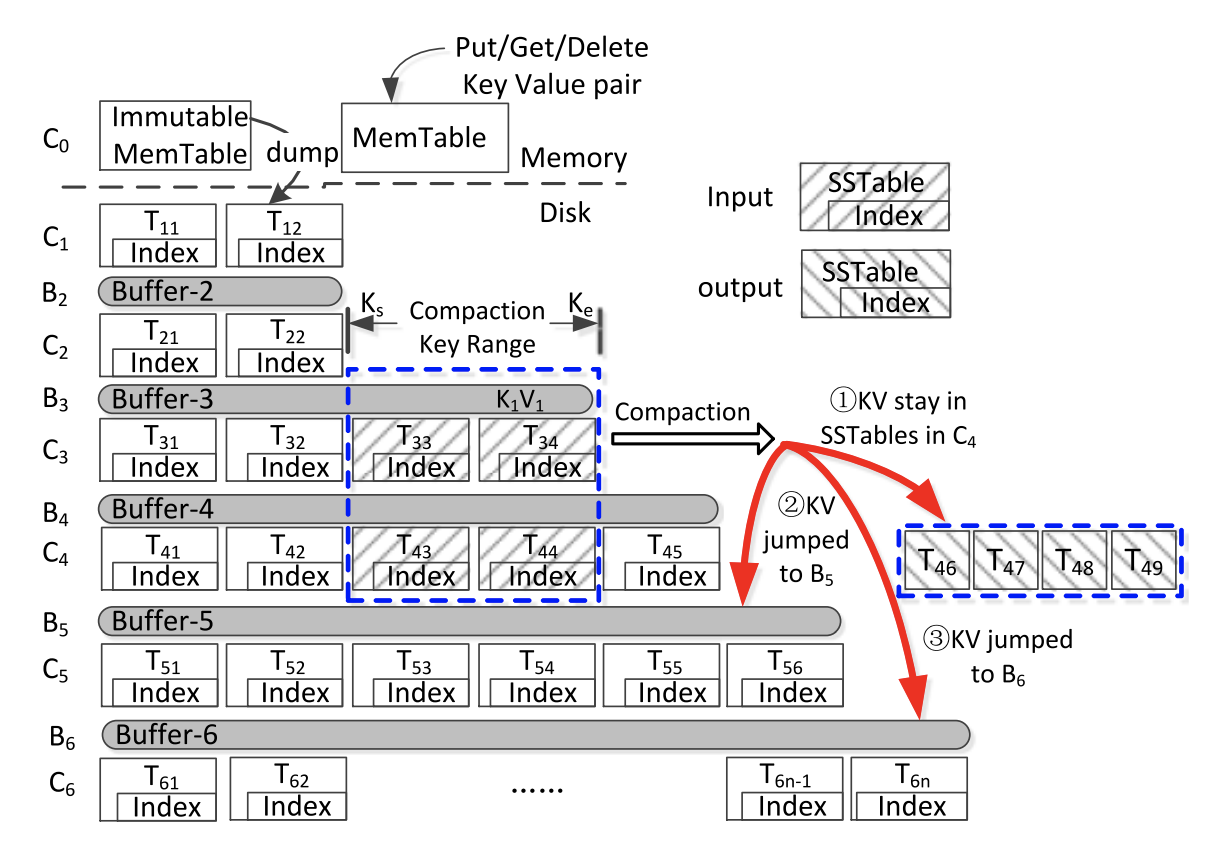
\includegraphics[scale=0.3]{Skip-tree.png}
    \caption{ The architecture of Skip-tree.}
    \label{fig:mesh1}
\end{figure}

\subsubsection{Disk Side optimization}
SMRDB \cite{SMRDB} is a KV data store that works specially for disks to address the need that to utilize disks by using approaches to leverage their proclivity for sequential writes as much as possible.
It aims at providing a new key-value data management for SMR disks to handle the overlapping data in random write and in-place updates operations on the disk.
SMRDB works as a KV database engine on the SMR disks. 
\par
The basic idea of SMR solution for LSM Tree is shown in Figure 4.
\begin{figure}[h]
    \centering
	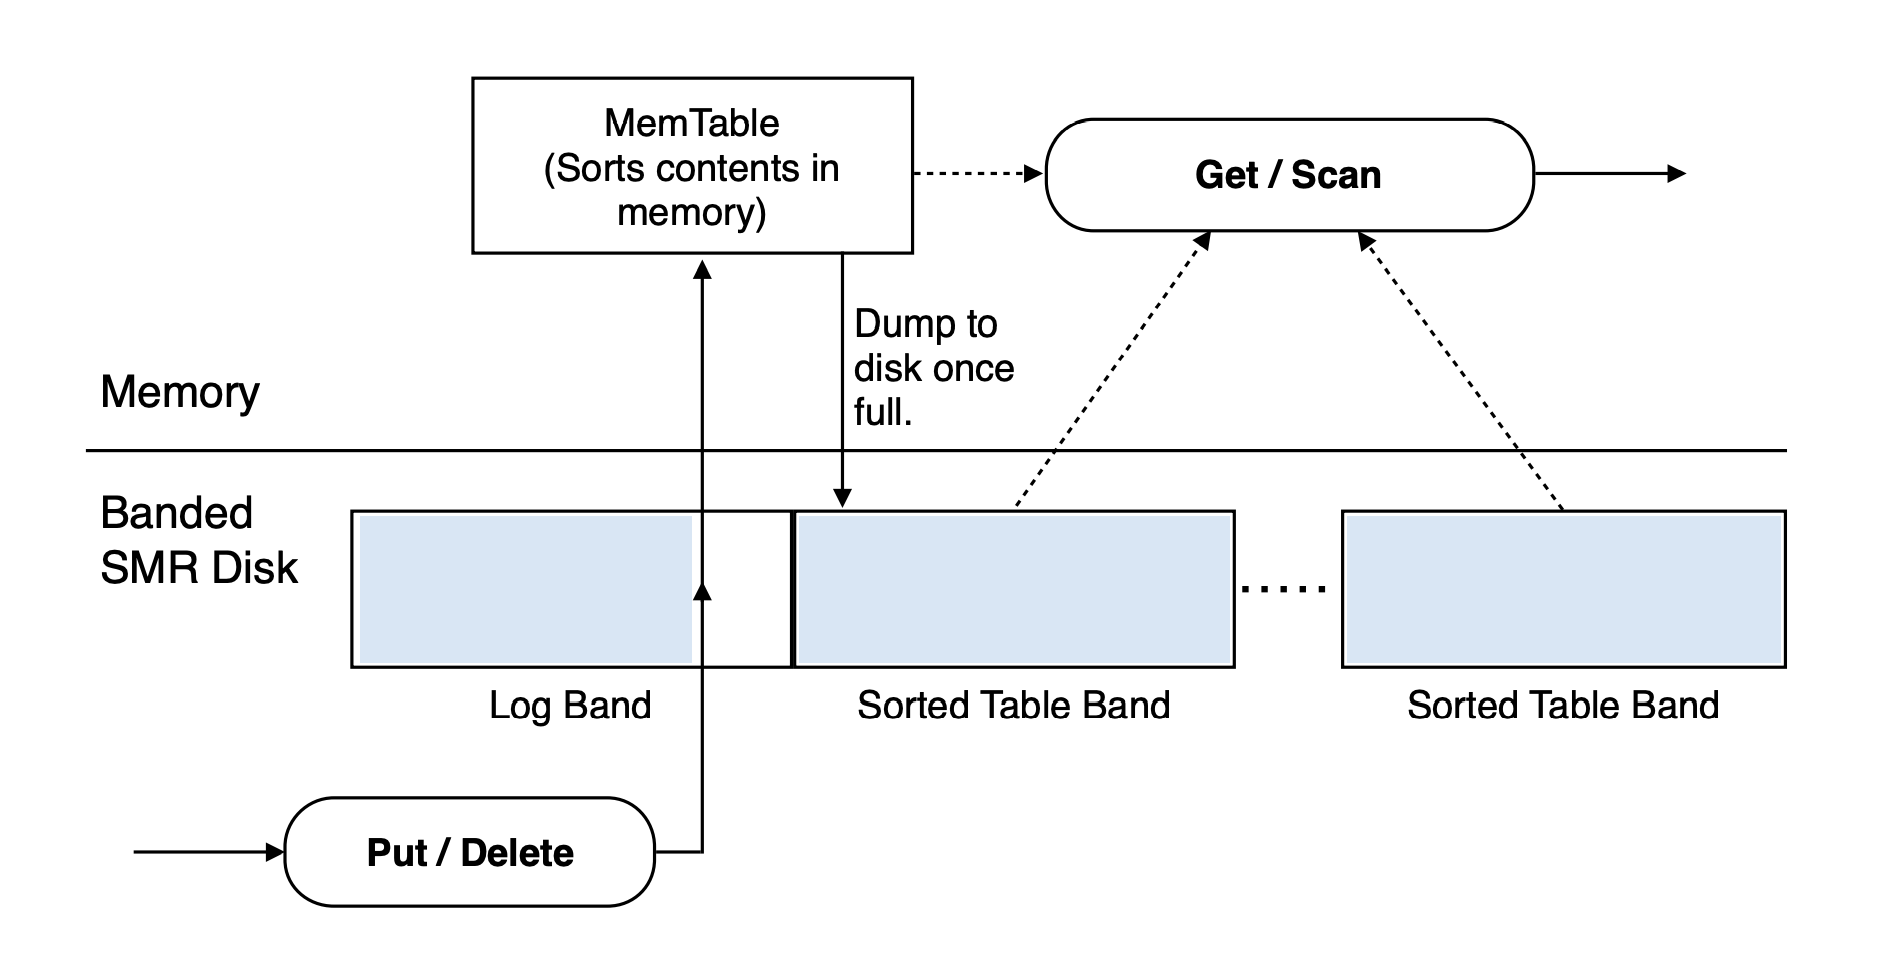
\includegraphics[scale=0.3]{SMR.png}
    \caption{ LevelDB based data access management.}
    \label{fig:mesh1}
\end{figure}
To meet the requirement of large data reorganization in LSM-Tree based databases, a simple SMR disks solution is introduced in this paper.
Stitching is used in the compaction process, where it basicly moves part of the compaction data to a new area, 
but some splited data will still remain in the same place and be stitched with in-coming new data.
But it can't be evaluated how this scheme works when compactions are carried in the background.



\subsection{Summary}
It can be shown from the previous work that skew will cause severe performance degradation, and the database system suffer from I/O brusts due to compaction and disk flushing.
MongoDB's solution to reduce skew is basically based on resharding and monitoring mechanism.
There are also many solutions that try to slove the I/O and CPU perfromance degradation.
But these three solutions above are mostly aimed at LSM-tree structure on individual nodes, they don't take the utilization of other nodes in consideration.
Hailstrom tries to solve these problems by disaggregate resources to address load balancing at database and storage layers seperately.

\section{Design of Hailstrom: Disaggregate Compute and Storage}

Hailstorm is designed to improve load balance and utilization for LSM-based distributed database.
It on a higher level to reduce the skew for read and write operations, as well as to reduce the I/O and CPU performace issue caused by compaction behavior.
The key idea of Hailstorm is to disaggregate compute and storage.

\subsection{Basic Architecture}
\par
The basic architecture of Hailstorm shown in Figure 5. 
Hailstorm works like a middleware in the middle of in-memory database storage instances and disk side storage devices.
The Hailstorm filesystem contains three parts:
1. Clients that provide filesystem interface to storage engines,
2. Servers that operate on local storages to store data and relavant operations,
3. Hailstorm agent in the middle to schedule operations of compaction tasks.

\begin{figure}[h]
    \centering
	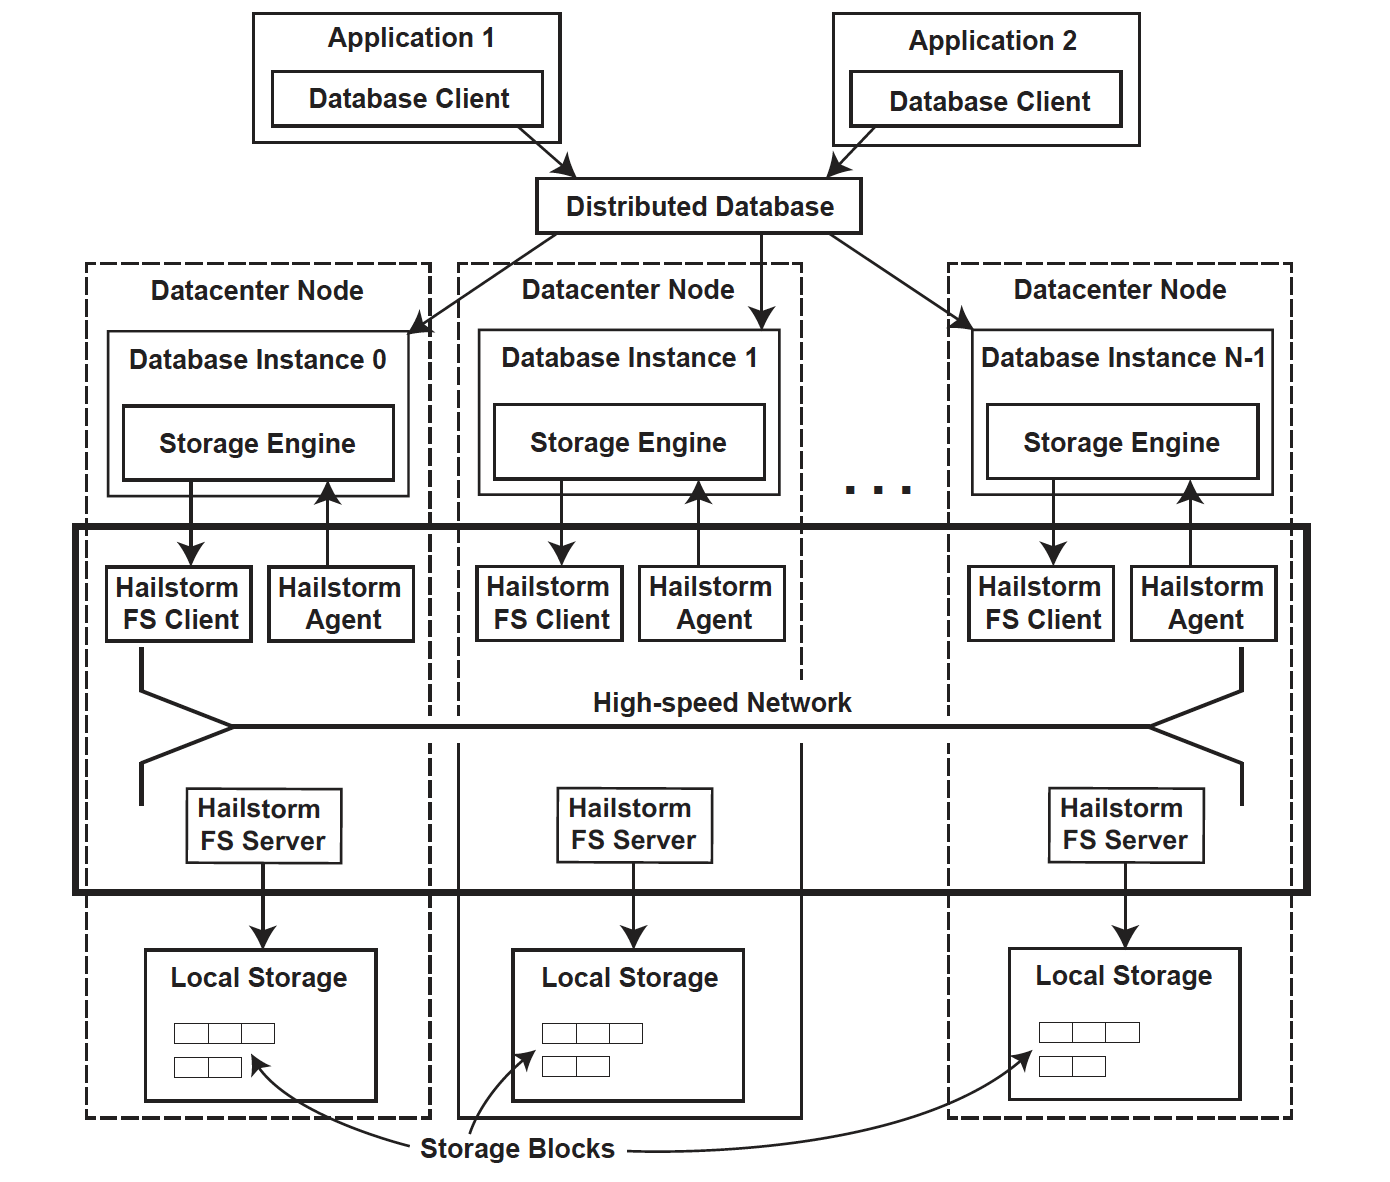
\includegraphics[scale=0.3]{Hailstorm2.png}
    \caption{ Distributed database deployed on a Hailstorm architecture.
	Hailstorm spreads data uniformly for each storage engine
	across all pooled storage devices within the rack.}
    \label{fig:mesh1}
\end{figure}

The user side operations could still operate on traditional databases. 

\subsection{Hailstorm Filesystem Interface}
\par
Hailstorm provides a subset of POSIX filesystem interface to storage engines rather than block-level interface.
As Hailstorm in the middle of local storage and database nodes, filesystem interface could provide filesystem-level informantion to sotrage engines.
Therefore Hailstorm sheilds KV store related specialized implementation details, and exposes traditional POSIX interface to nodes.
\par
In order to promote I/O performance, Hailstorm filesystem keeps most metadata locally and use smaller block size compared with traditional LSM-based databases.
The filesystem is also designed specially to reduce the influence of compaction, and aggresive prefetching is carried out to compaction tasks.

\subsection{Storage Architecture Design}
\par
In order to provide disaggregation of computation and storage, the storage architecture of Hailstorm is designed to pool all data from nodes in a large rack.
In the large rack, data is divided into small blocks (typically 1MB), which is designed in this way to reduce I/O latency and throughput in compaction.
In this way, LSM storage could avoid flush stalls in compaction. 
Another advantage of this approach is that as long as the bandwidth is wide enough, Hailstorm could work on the whole-rack level, 
therefore there's no need nof locality consideration.
The splited data blocks are spreaded uniformly to database servers. 
In read operation, data could be accessed evenly, therefore there's no need to spend additional time for searching the position of data, as the locations are certain.
The client would automatically prefetches blocks to promote the performace.
\par
Load balancing is an important goal of Hailstorm. 
As data blocks are splited uniformly on different servers, load balancing can be well guaranted as it avoids the centralized data index management.
Specifically, imbalance among servers are reduced in 2 ways.
\begin{displayquote}
	First, the pseudorandom
	mapping M is a function of the file path (as denoted
	previously byMF ), which ensures that different clients working
	on different files do not operate in lockstep. Second, we
	use batch sampling to ensure high storage utilization by ensuring
	there are always multiple pending operations.
\end{displayquote}
Another goal of Haistorm is to improve the performance.
In the part of storage design, this is achieved by prepatching. 
Besides, in order to promote read performance, Hailstorm will have reads from previous threads at smaller block granularity.

\subsection{Compaction Offloading}
\par
In the previous section, compaction offloading is disscussed, that by splitting data into small blocks, seperating blocks uniformly across servers, 
and using aggresive pre-fetching mechanism, the performace influence of compaction could be reduced.
In this section, specialized mechanisms are applied for compaction offloading.
That is, generally, outsourcing compaction tasks to other machines.
\par
A lightweight backgroud agent is running to monitor the data usage situation. 
The monitor process will detect if I/O or CPU resources are overload due to compaction.
Hailstorm will then decide heuristicly whether to offload local compaction tasks, and in this way to balance CPU load within a rack over time.


\section{Evaluation}

The goal of the evaluation is to judge the performance of Hailstorm on these aspects:
\begin{displayquote}
1. How do distributed databases perform when deployed
on Hailstorm in terms of throughput and latency, especially
in the presence of skew? 
\newline
2. Does resharding help in traditional deployments? How
does it compare with Hailstorm?
\newline
3. Can databases supporting distributed SQL transactions
benefit from using Hailstorm? 
\newline
4. What is the impact of different features of Hailstorm
on performance and how does it compare with other
distributed filesystems such as HDFS? Do configuration
values affect performance? Can Hailstorm
improve throughput for B-trees?
\end{displayquote}
Here we mainly focus on the performance of Hailstorm in sloving skew problem and compaction performance degradation.
The benchmark is carried out on MongDB.
The basic workflow to test how Hailstorm performs on solving skew is as following.
Yahoo! Cloud Serving Benchmark (YCSB) is used to run the benchmark.
YCSB provides 6 different senarios from YCSB A to YCSB F, and the paper add some other senarios in addition.
The test workload table is shown in Figure 6.
\begin{figure}[h]
    \centering
	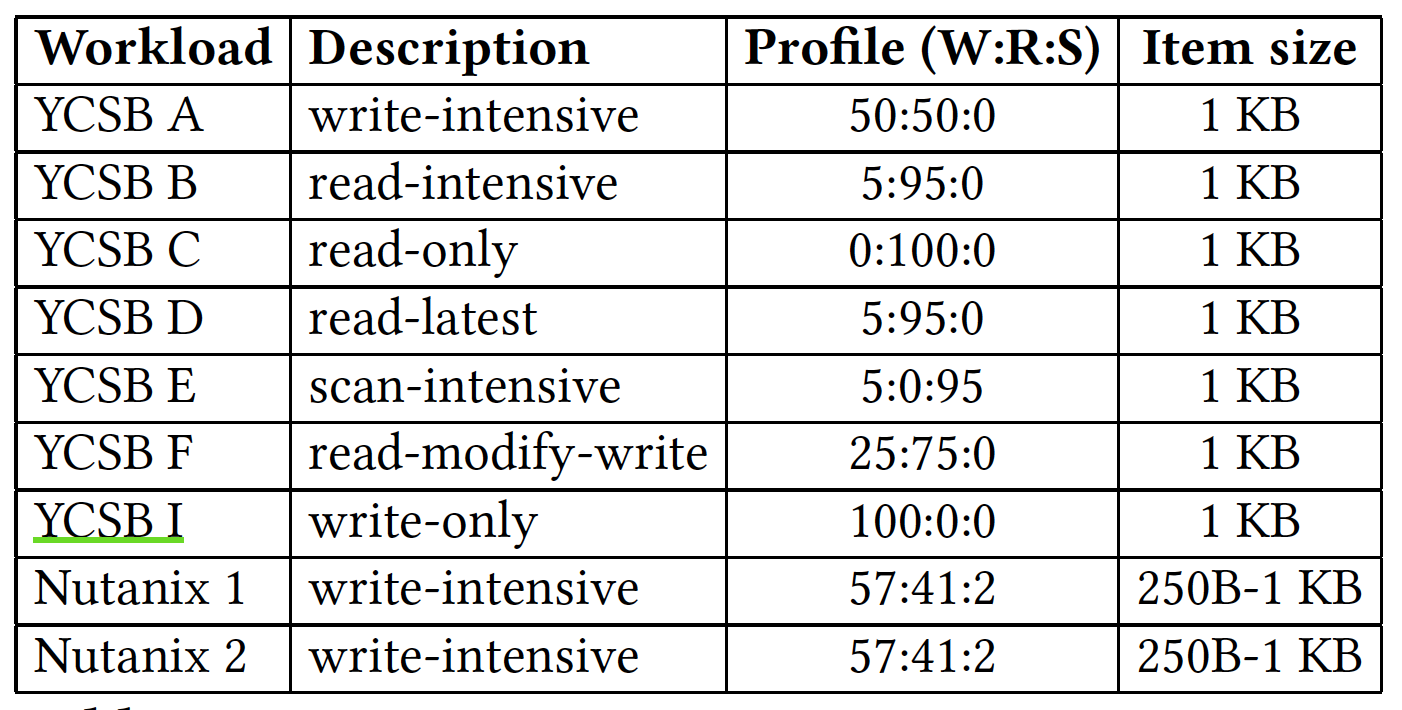
\includegraphics[scale=0.3]{YCSB_workload.png}
    \caption{MongoDB workloads description and characteristics}
    \label{fig:mesh1}
\end{figure}
\begin{displayquote}
	We first populate the database with 100 GB of data (100
	million keys) from each workload before executing the workload
	with an additional 100 GB of data (100 million keys).
	We execute Nutanix’s workloads with a pre-populated database
	containing 256 GB of data, and execute each workload
	with an additional dataset size of 256 GB (approximately 700
	million keys).
\end{displayquote}

\begin{figure}[h]
    \centering
	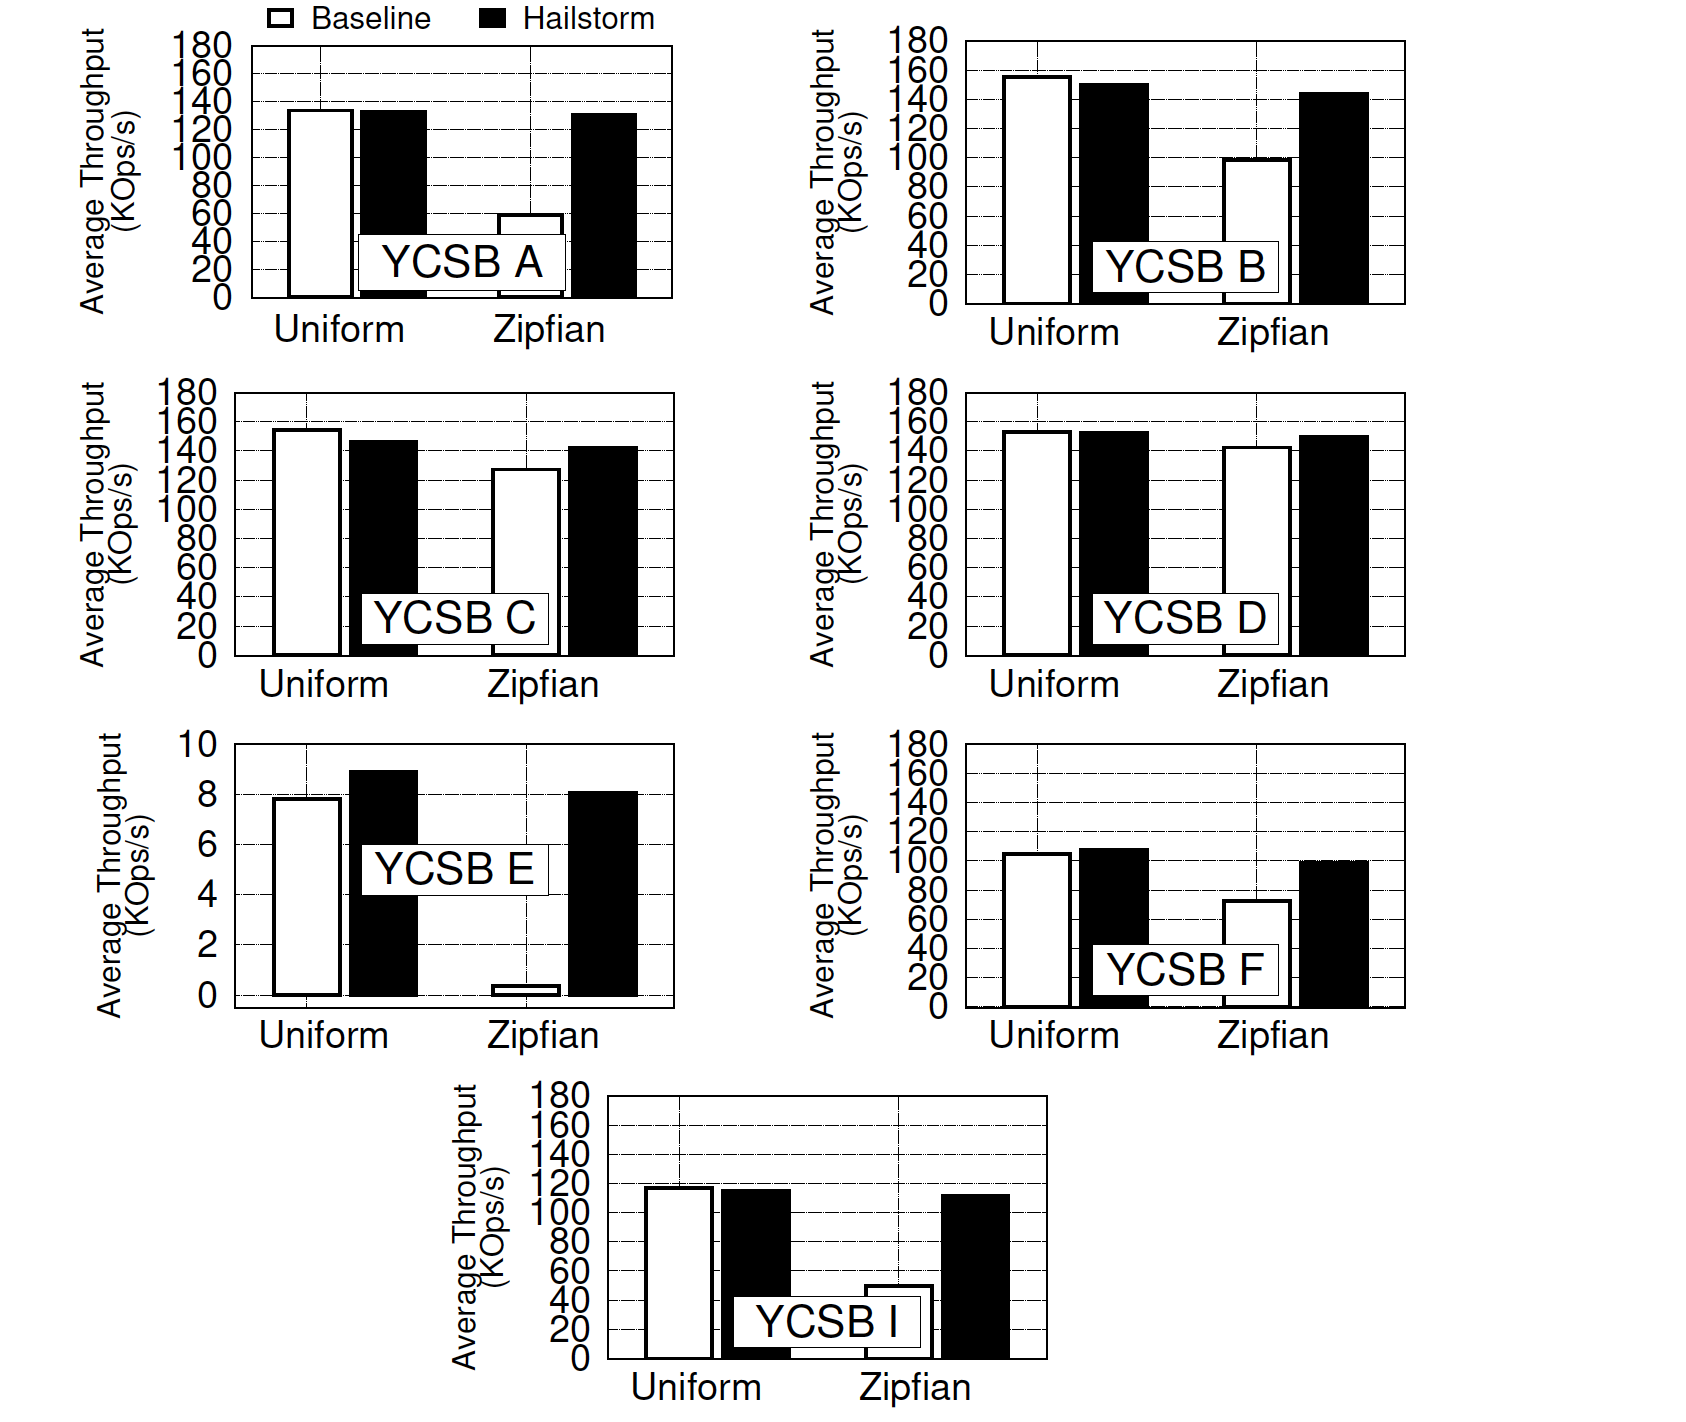
\includegraphics[scale=0.3]{YCSB_throughput.png}
    \caption{MongoDB average throughput for Baseline and Hailstorm
	for YCSB workloads with uniform and Zipfian key distributions.
	Hailstorm maintains high throughput on all workloads.}
    \label{fig:mesh1}
\end{figure}
As is shown in Figure 7, Hailstorm performs better than Baseline in throughput in handling Zipfan data, where there are more skews in the data set.
In dealing with Uniform data, Hailstorm performs almost the same with the Baseline, and there are slightly more overheads in some senarios than the Baseline.
\par
Hailstorm is also tested with TiDB to see how it performs against compactions.
TPC-C\cite{10.1145/369275.369291} benchmark and TPC-E\cite{10.1145/1942776.1942778} benchmark are carried out.
It compares the throughput (measured in transactions per second) over a period of time of 1 hour for both scenarios and both benchmarks. 
The result is shown in Figure 8.
It can be concluded from the result that generally Hailstorm has a better performance in reducing performace degradation caused by compactions.
Baseline suffers from compaction, as after a period of time, the throughput will decrease continuously due to the operation of compaction on TiKV instances and resharding operations.
Hailstorm performs more stablily in the exsistence of skew. 
The compaction offloading helps to drop some compaction tasks on certain nodes, and ensures a stable throughput in general.

\begin{figure}[h]
    \centering
	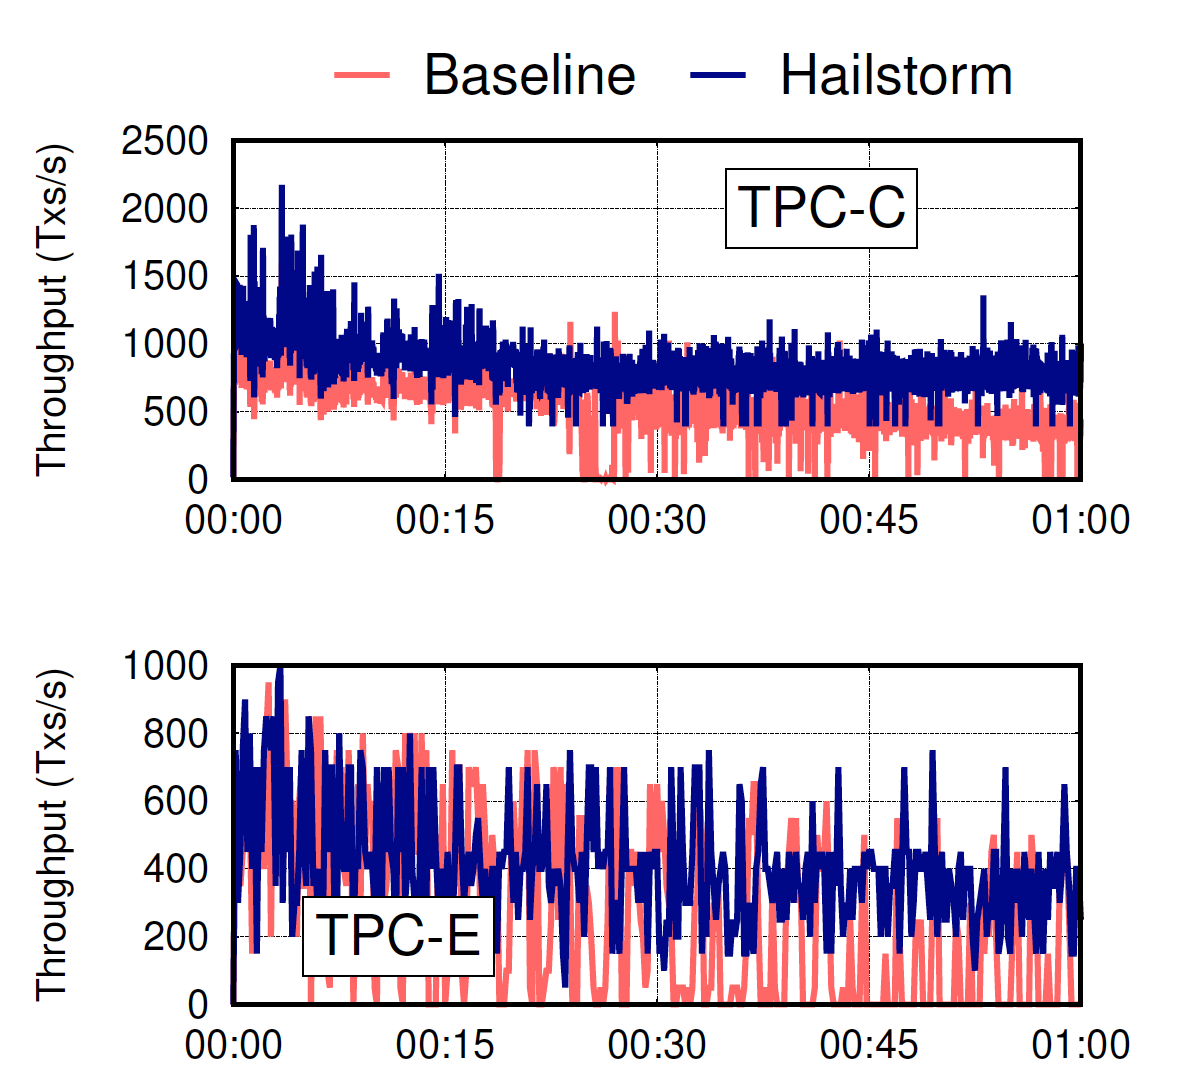
\includegraphics[scale=0.3]{TiDB_result.png}
    \caption{TiDB per 10-second throughput timelines (HH:mm)
	for Baseline and Hailstorm with TPC-C and TPC-E.}
    \label{fig:mesh1}
\end{figure}


\section{Discussion}

What is bad about your paper? 
What are the good points? 
Mention criticism and ideas for improvement that you thought about while researching the topic.

\section{Conclusion}

Sum up your paper and the discussion points.

\bibliographystyle{unsrt}
\bibliography{handin} 

\end{document}
